\section{Results}
\label{sec:results}

In this section, we present the results of the different statistical methods we applied in our our dataset (Section~\ref{sec:data_set}). We have divided our findings in three different subsections for better understanding: \textit{Number of collaborations}, \textit{Impact in research outcomes} and \textit{Researched Topics}.

\subsection{Results for the Number of collaborations}

As we can see in Table \textit{\ref{table:num_of_publications}}, the nation that published the highest number of publications was the US (835.456) followed by the EU (727.151) and lastly China (692.924). If we look into the number of journal articles written as a result of a collaboration between the regions, we can see that the EU and the US were the territories that collaborated the most, having a total of 84.701 publications done together. It is followed by the number of collaborations between the US and China (73420), China and the EU (26267), and finally, the least common collaboration was between the 3 regions (3277).

\begin{table}[]
    \centering
    \begin{tabular}{lcccccccc}
    \hline
    \multicolumn{1}{c}{Collaboration type} & CN-only & EU-Only & US-Only & CN-EU & CN-US & EU-US & CN-EU-US & Total   \\ \hline
    All                                    & 692924  & 727151  & 835456  & 26267 & 73420 & 84701 & 3277     & 2443196 \\
    Education                              & 672256  & 678427  & 748132  & 24024 & 65978 & 68861 & 2648     & 2260326 \\
    Company                                & 4064    & 16015   & 31420   & 92    & 153   & 1375  & 9        & 53128   \\
    Mixed                                  & 16604   & 32709   & 55904   & 2151  & 7289  & 14465 & 620      & 129742  \\ \hline
    \end{tabular}
\caption{Number of publications per collaboration type}
\label{table:num_of_publications}
\end{table}

In all the cases, the co-authorship between authors from the same region represents more than 70\% of their total co-authored articles as shown in Table \textit{\ref{table:collaboration_percentage}}. However, China has the highest rate, with a 76.75\% of their collaborations only within the country. It is followed by the US with 71.33\% of self-collaboration and finally the EU with 71.15\%. These results suggest that China has been more isolated in terms of collaboration opportunities than the others. It can also be observed in the importance the different countries have given to the others. Both the EU and the US have prioritized each other. Thus, the number of co-authored papers published between the EU and the US represents 8.29\% of the total published papers for the EU, and 7.23\% for the US, while collaborations with China represent 2.57\% of the total for the EU and 6.27\% for the US. It also suggests that China has prioritized collaborating with the US. Collaborations between the three regions have been minoritarian for all of them, with rates between the 0.28\% for the US the 0.36\% for China. We have analyzed the impact of the collaboration type, that is if the collaboration was between educational institutions, companies, or both. Although the collaboration patterns remain equal in all cases, when collaboration is done between public and private institutions, the internationalization rate is higher. 

\begin{figure}[tb]
    \centering
    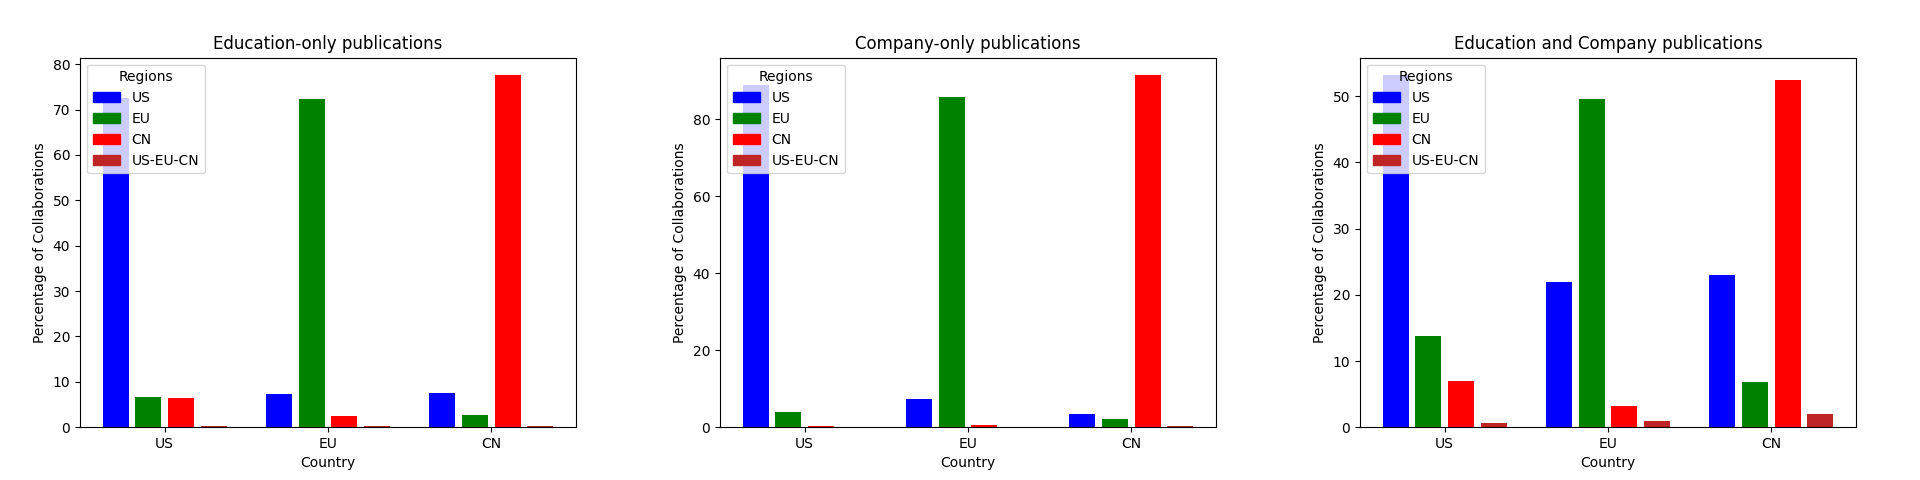
\includegraphics[width=0.8\textwidth]{images/collaboration_percentage_by_collab_type.png}
    \caption{Collaboration percentage by collaboration type}
    \label{fig:collaboration_percentage_by_collab_type}
\end{figure}

In in Figure \ref{fig:collaboration_percentage_by_collab_type}, we can observe how the countries go from 77.56\%, 72.38\%, and 72.58\% of self-collaboration for China, the EU, and the US respectively in the case of education-only co-authorship to a rate of 52.48\%, 49.52\%, and 53.17\% in the case of collaborations between mixed institution types. In addition to this, the percentage of papers published in collaboration with institutions from the US increased either for China or the EU, going from 7.61\% and 7.35\% for China and the EU in the case of educational institutions only, to 23.04\% and 21.90\% in the cases of mixed institution types.

\begin{table}[]
        \centering
    \begin{tabular}{lcccc}
    \hline
    Country & With CN & With EU & With US & All 3 regions \\ \hline
    CN      & 76,75\% & 2,91\%  & 8,13\%  & 0,36\%        \\
    EU      & 2,57\%  & 71,15\% & 8,29\%  & 0,32\%        \\
    US      & 6,27\%  & 7,23\%  & 71,33\% & 0,28\%        \\
            &         &         &         &               \\ \hline
    \end{tabular}
    \caption{Relative collaboration rates per country}
    \label{table:collaboration_percentage}
    \end{table}

Although in a long-term perspective the EU and the US were the most productive regions in terms of the number of papers published, in Figure \ref{fig:collaborations_between_countries_per_year} we can observe that China became the most published country in 2017, followed by the EU and the US. Regarding the articles published in collaboration, the EU and the US used to be the most productive duple, but in 2014, China and the US surpassed the previous couple, becoming the two most productive publishers as we can see in Figure \ref{fig:collaborations_between_countries_per_year}. The number of co-authored articles between China and the EU has been also increasing, having a positive tendency, similar to the one noted during the last 5 years between China and the US. Finally, we can observe that the number of collaborations between the three territories has been also increasing, especially since 2015.

\begin{figure}[tb]
    \centering
    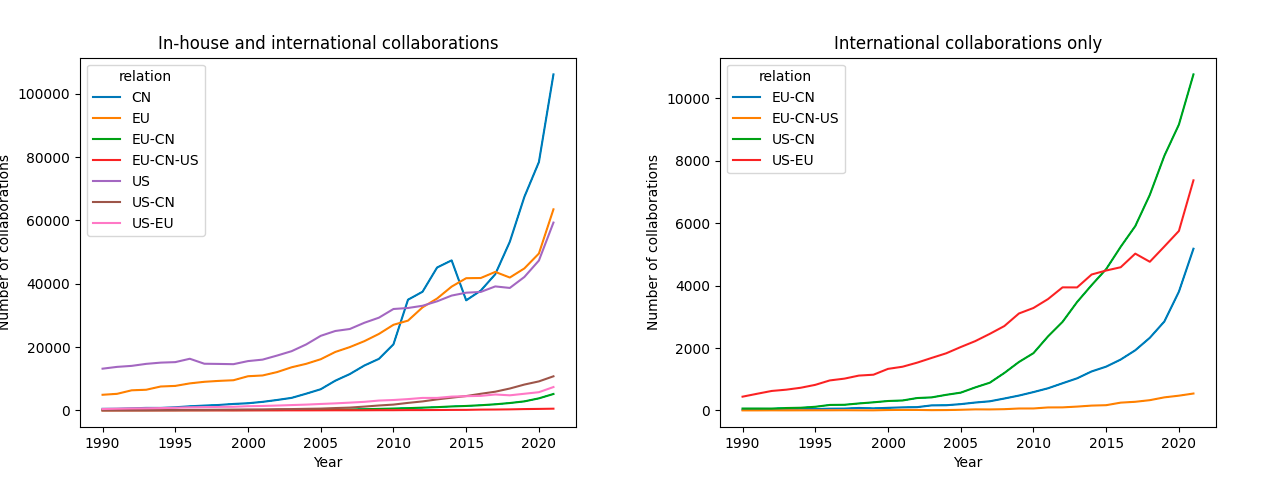
\includegraphics[width=0.8\textwidth]{images/collaborations_between_countries_per_year.png}
    \caption{Collaboration percentage by collaboration type}
    \label{fig:collaborations_between_countries_per_year}
\end{figure}

\subsection{Results for the Impact in research outcomes}

\begin{table}[]
    \centering
    \begin{tabular}{lcccccccc}
    \hline
    Collaboration type & CN-only & EU-Only & US-Only & CN-EU & CN-US & EU-US & CN-EU-US & AVG   \\ \hline
    All                & 13,32   & 21,64   & 37,24   & 24,14 & 27,89 & 38,12 & 32,88    & 27,89 \\
    Education          & 13,41   & 21,84   & 37,41   & 24,44 & 27,83 & 38,86 & 32,66    & 28,06 \\
    Company            & 6,41    & 15,4    & 31,95   & 19,59 & 15,87 & 17,8  & 11,11    & 16,88 \\
    Mixed              & 11,43   & 20,56   & 38,04   & 21,04 & 28,64 & 36,53 & 34,12    & 27,19 \\ \hline
    \end{tabular}
\caption{Average number of citations per collaboration type}
\label{table:avg_citations_by_collab_type}
\end{table}

Apart from the articles themselves, we have measured the number of citations as the outcome of the published articles. In an overall comparison, we found that the papers published through the collaboration between the EU and the US obtained the highest citation rate with an average of 38.12 citations per paper as we can see in Table \textit{\ref{table:table_avg_citations_by_collab_type}}. It´s followed by publications done by the US only with a 37.24 citation average, and by the publications where the three regions worked together with 32.88 average citations. The rest of the results are below an average of 30 citations per research paper, the least cited papers were those published only by Chinese institutions, with an average of 13.32 citations per paper, far from the second least cited publications, the EU only with an average of 21.64. However, China increased its rates by collaborating with the US and the EU, which also helped the EU to increase its own rates. Therefore, the collaboration between China and the US brought an average of 27.89 citations, as well as the collaboration between China and the EU brought an average of 24.14 citations, increasing their country-only rates for both regions, China and the EU. 
If we take a deeper look at the average number of citations between the actors across the different collaboration types, we see that those papers written by authors belonging to private companies had the least number of citations, with an average of 16.88, being China especially disadvantaged, with an average of 6,41 citations per paper, suggesting that publications from Chinese companies do not get relevance in academic research.

\begin{table}[]
    \centering
    \begin{tabular}{lcccccc}
    \hline
                       & CN         &                  & EU         &                  & US         &                  \\ \cline{2-7} 
    Collaboration type & \textit{r} & \textit{p-value} & \textit{r} & \textit{p-value} & \textit{r} & \textit{p-value} \\ \hline
    Education          & -0,18      & \textless{}.05   & -0,06      & \textless{}.05   & -0,01      & \textless{}.05   \\
    Company            & -0,14      & \textless{}.05   & 0          & 0,63             & 0,07       & \textless{}.05   \\
    Mixed              & -0,19      & \textless{}.05   & 0,01       & 0,04             & 0,08       & \textless{}.05   \\
    All                & -0,18      & \textless{}.05   & -0,06      & \textless{}.05   & 0          & \textless{}.05   \\ \hline
    \end{tabular}
\caption{Spearman Correlation Test results for the number of citations and the participation ratio per collaboration type}
\label{table:correlation_test_citations_participation_ratio}
\end{table}

We also analyzed how the number of participants from each region affect the final number of citations. To measure it, we compute the number of participants from a region over the total number of participants in the paper, obtaining a participation ratio. Then we used the Spearman Correlation Rank test to analyze if there is a correlation between the country participation ratios and the number of citations obtained. In Table \textit{\ref{table:table_table_correlation_test_citations_participation_ratio}}, we can see that the number of institutions from the US participating in the research article may not have an impact on the total number of citations. On the other hand, results suggest that there might be a weak negative correlation between the number of Chinese or European institutions participating in the research and the final number of citations. While for the UE, Spearman’s rank correlation between the two variables is -0.06 with a corresponding p-value of <0.05, for China this coefficient is three times higher, with a corresponding p-value of <0.05. Focusing on the different co-authorship types, we found that China had negative correlation values in all cases, the highest of those occurring in collaborations between Chinese companies and public institutions, where there was a negative correlation between the two variables, r (31641) = -0.19, p = <0.05. On the other hand, the EU had no significative correlation results in all cases but education, where it obtained a negative correlation of -0.06 with a corresponding p-value of <0.05. Finally, the US obtained positive correlation results in the collaborations between companies and between companies and public institutions, obtaining a positive correlation of -0.07 with a corresponding p-value of <0.05 and a positive correlation of -0.08 with a corresponding p-value of <0.05 respectively.

\subsection{Results for Researched Topics}

We have obtained the keywords of every publication, and we have listed the overall top 10 most used terms for every collaboration type between the regions. As we can see in Figure \ref{fig:topics_all_relations}, in China and the UE, as well as in their collaborations between them and the US, some topics have grown more than others. China seems to be prioritizing “Artificial Intelligence”, “Physics”, “Mathematics”, and “Engineering” over the others. Therefore, these topics have become the most published in internal collaborations, but China is also pushing these topics when working with international colleagues, raising these 4 topics in their collaborations with the EU and the US. Within these topics, the results suggest that China is particularly focusing on “Artificial Intelligence”, which is a topic that is being more researched in the last few years. Internal collaborations within the EU also have those 4 topics as the most researched. However, the EU is not only focusing on artificial intelligence. In contrast to the Chinese case, the EU patterns are not repeated when collaborating with the US, being in this case less grouped. The US does not have the clustering tendency we observed in the others. Although they are also researching more in “Artificial Intelligence”, it seems that they are also working on other fields such as “Psychology” or “Medicine”, relating them to the topic “Computer Science”. These topics are also observed when the US works with the EU, but not with China, suggesting that these are fields that may be more interesting for both.

\begin{figure}[tb]
    \centering
    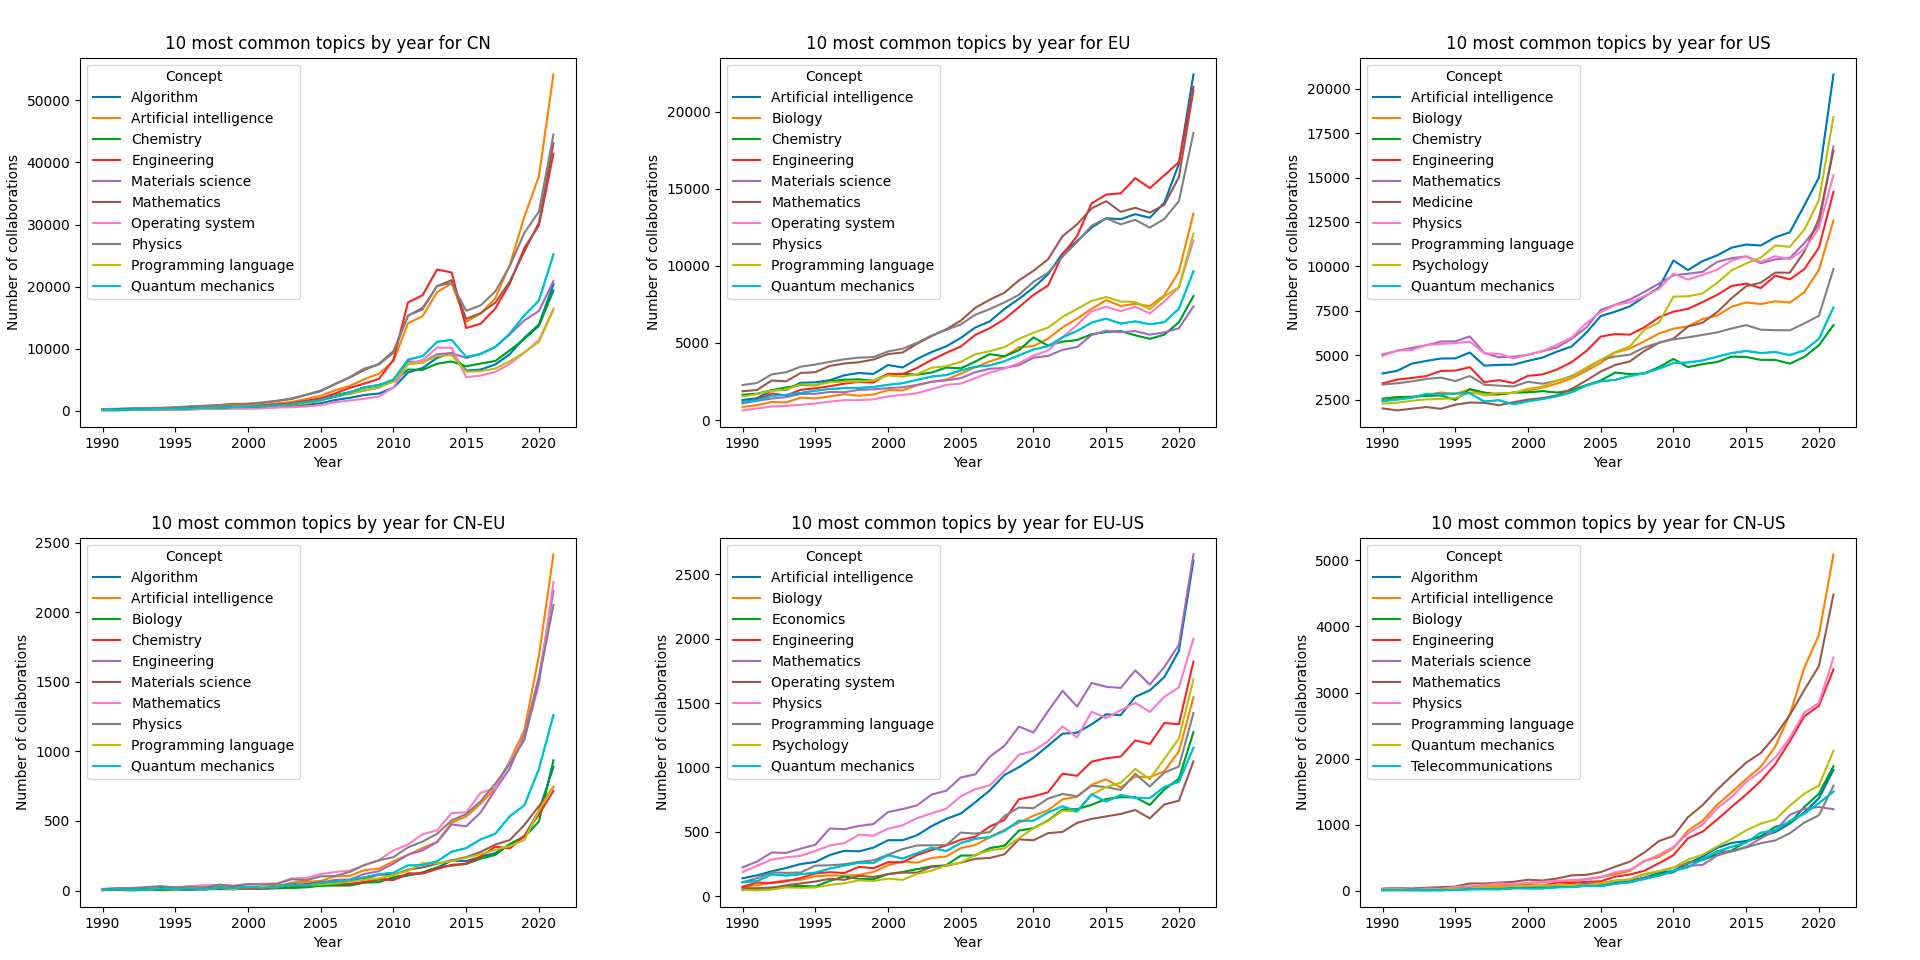
\includegraphics[width=0.8\textwidth]{images/topics_all_relations.png}
    \caption{Most researched topics by collaborating regions}
    \label{fig:topics_all_relations}
\end{figure}